\section{Chapter 6: The Hydrogen Bomb}

\subsection{Give a historical international perspective on the development of the H-bomb.}
\begin{multisolutionblock}
Some isotopes of uranium and plutonium have nuclei that are so close to being unstable that they fragment and release energy when bombarded with neutrons. A fission chain reaction builds up because each fragmenting nucleus produces several neutrons that can initiate further reactions. An explosion occurs if the piece of uranium or plutonium exceeds a certain critical mass — thought to be a few kilograms (i.e., smaller than a grapefruit). In order to bring about the explosion, this critical mass has to be assembled very quickly, either by firing together two subcritical pieces or by compressing a subcritical sphere
using conventional explosives. The US developed the first atom bombs in
great secrecy during World War II at Los Alamos, New Mexico. The first test weapon, exploded in New Mexico in July 1945, had a force equivalent to 21 kilotons of high explosive. A few days later, bombs of similar size devastated the Japanese cities of Hiroshima and Nagasaki.
\textbf{Producing the fissile materials for such weapons was difficult and expensive and required an enormous industrial complex. Less than 1 \% of natural uranium is the “explosive” isotope 235U, and separating it from the more abundant 238U is very difficult}. Plutonium does not occur naturally at all and must be manufactured in a fission reactor and then extracted from the intensely radioactive waste. Moreover, the size of a \textbf{pure fission bomb was limited by the requirement that the component parts be below the critical mass. Fusion does not suffer from this size limitation and might allow bigger bombs to be built. The fusion fuel, deuterium, is much more abundant than 235U and is easier to separate}.
Even as early as 1941, before he had built the very first nuclear (fission) reactor in Chicago, the physicist Enrico Fermi speculated to Edward Teller that \textbf{a fission bomb might be able to ignite the fusion reaction in deuterium in order to produce an even more powerful weapon}—this became known as the \textbf{hydrogen bomb}, or \textbf{H-bomb}. These ideas were not pursued seriously until after the war ended. Many of the scientists working at Los Alamos then left to go
back to their academic pursuits. Robert Oppenheimer, who had led the development of the fission bomb, resigned as director of the weapons laboratory at Los Alamos to become director of the Princeton Institute of Advanced Study and was replaced by Norris Bradbury. Edward Teller, after a brief period in academic life, returned to Los Alamos and became the main driving force behind the development of the H-bomb, with a concept that was called the \textbf{Classical Super}.

There was, however, much soul-searching in the US as to whether it was
justified to try and build a fusion bomb at all. In 1949, Enrico Fermi and Isidor Rabi, both distinguished physicists and Nobel Prize winners, wrote a report for the Atomic Energy Commission in which they said:

\textit{Necessarily such a weapon goes far beyond any military objective and enters the range of very great natural catastrophes…. It is clear that the use of such a weapon cannot
be justified on any ethical ground which gives a human being a certain individuality and dignity even if he happens to be a resident of an enemy country…. The fact that no limits exist to the destructiveness of this weapon makes its existence and the knowledge of its construction a danger to humanity as a whole. It is an evil thing considered in any light.}
\newpage

The debate was cut short in early 1950 by the unexpected detonation of
the first Soviet fission bomb. Prompted by the suspicion that East German spy Klaus Fuchs had supplied information about US hydrogen-bomb research to the Soviet Union, President Truman ordered that the Super be developed as quickly as possible. However, no one really knew how to do this, so new fears were raised that Truman’s statement might simply encourage the Soviet Union to speed up its own efforts to build a fusion bomb and, more seriously, that the Soviet scientists might already know how to do it.
\end{multisolutionblock}

\subsection{Explain the requirement for a H-bomb and advantages over pure fission.}
\solutionblock{see above}

\subsection{Discuss limited resources and processing for Uranium and Tritium.}
\solutionblock{There were further serious problems in terms of providing the fusion fuel. A mixture of deuterium and tritium would ignite most easily, but \textbf{tritium does not occur naturally and must be manufactured in a nuclear reactor}. A DT fusion bomb with an explosive yield equal to that of 10 million tons of TNT (10 megatons) would require hundreds of kilograms of tritium. The rough size of the bomb can be estimated from the density of solid deuterium; it would be equivalent to a sphere about 1 meter in diameter. Smaller quantities of deuterium and tritium could be used to boost the explosive force of fission bombs or to initiate the ignition of a fusion weapon. But to manufacture tritium in the
quantities needed for a significant number of pure DT bombs would require
a massive production effort—dwarfing even the substantial program already
under way to manufacture plutonium—and would be prohibitively expensive.

For Uranium, the problem is that \textbf{less than 1 \% of natural uranium is the “explosive” isotope 235U, and separating it from the more abundant 238U is very difficult} (see above).
}

\subsection{How does an H-bomb in the Teller-Ulam design work? Draw and explain.}

\begin{multisolutionblock}
    
Due to the reasons mentioned above, Teller created a new idea, which didn't work. With the help of Ulam they created the Teller-Ulam design:

Early in 1951, Ulam made an important conceptual breakthrough, and
Teller quickly refined the idea. This followed an idea known as radiation
implosion that had first been broached in 1946 by Klaus Fuchs before he was arrested for giving atomic secrets to the Soviet Union. Most of the energy leaves the fission trigger as X-rays. Traveling at the speed of light, the X-rays can reach the nearby fusion fuel almost instantaneously and be used to compress and ignite it before it is blown apart by the blast wave from the fission explosion, which travels only at the speed of sound. This is analogous to the delay between seeing a flash of lightning and hearing the sound of the thunder, though the much smaller distances in the bomb reduce the delay to less than a millionth of a second. A second important requirement is that the radiation from the fission bomb needs to compress the fusion fuel before it is heated to the high temperature at which it will ignite. It is much easier to compress a gas
when it is cold than when it is hot.

\begin{figure}[H]
    \centering
    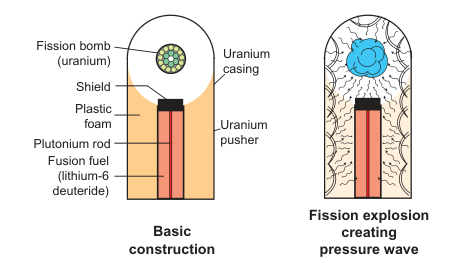
\includegraphics[width=0.75\textwidth]{chapters/fig/6_teller.png}
    \caption{Schematic diagram of the elements of an H-bomb. A fission explosion is first triggered by high explosive. This explosion is contained inside a heavy metal case. The radiation from
    the fission bomb causes the implosion and heating of the fusion fuel and sets off the fusion bomb.}
    \label{fig:6_teller}
\end{figure}
    
    
The fission bomb trigger is set off at one end of a cylindrical casing in
which the fusion fuel is also contained. The fusion fuel is thought to be in the form of a cylinder surrounding a rod of plutonium, and a layer of very dense material—usually natural uranium or tungsten—surrounds the fuel itself. The X-ray radiation from the fission bomb is channeled down the radial gap between the outer casing and the fusion fuel cylinder. The gap is filled with plastic foam that is immediately vaporized and turned into hot plasma. The plasma is transparent to the X-rays, allowing the inner surface of the cylindrical casing and the outer surface of the dense layer surrounding the fusion fuel to be heated quickly to very high temperatures. As the outer surface of the layer surrounding the fuel vaporizes, it exerts a high inward pressure—rather
like an inverted rocket engine.

Enormous pressures are generated instantaneously—several billion times
atmospheric pressure—and the fuel is compressed to typically 300 times its
normal density. It is salutary to realize that the explosive force released by the fission trigger, enough to destroy an entire city, is being used briefly to squeeze a few kilograms of fuel! The compression and the neutrons from the fission bomb cause the plutonium rod down the middle of the fusion fuel to become critical and to explode—in effect a second fission bomb goes off. This explosion rapidly heats the already compressed fusion fuel to the temperature required for the fusion reactions to start. Once ignited, the fusion fuel burns outward and extremely high temperatures—up to 300 million degrees—are reached as almost the whole of the fuel is consumed. Some reports suggest
that the design has been refined so much that the plutonium “spark plug” is no longer needed.
\end{multisolutionblock}

\subsection{Discuss ideas for civil uses of nuclear bombs and why they failed.}
\solutionblock{

\textbf{Project Plowshare (USA)}: The
project considered civil engineering applications, such as \textbf{using a series of nuclear explosions to either widen the existing Panama Canal or to construct a new sea-level waterway connecting the Atlantic and Pacific oceans, to construct new dams and harbors and to cut railroads and highways through mountainous areas}. Other ideas involved blasting underground caverns for \textbf{storing water, natural gas, or petroleum and using underground explosions to improve the flow from difficult oil or natural gas fields} by fragmenting rock formations
that have low natural permeability. The US carried out nearly thirty underground explosions during the 1960s and '70s to study some of these ideas,
but \textbf{Project Plowshare was ended in 1977 due to growing concerns about radioactive fallout and about the ethics of using nuclear weapons under any circumstances}.
\\
\\
\textbf{Energy convertion}: One peaceful application studied in the United States was the possibility of converting the energy released by a nuclear explosion into electricity. The simplest idea was to set off a small nuclear bomb deep underground inside a natural formation of rock salt. The energy of the explosion would melt the
salt—and then water would be pumped into the cavity and the steam extracted to generate electricity. This concept was tested in December 1961 in the first explosion of the Plowshare series—a test known as Gnome using a small fission bomb with a yield of about 3 kilotons.
\\
\\
\textbf{Project Pacer}: The concept was followed up in the mid-1970s at Los Alamos National Laboratory with a study (known as the Pacer Project) of a more sophisticated scheme to \textbf{generate a steady supply of electricity from nuclear explosions}. A typical design envisaged exploding the bombs inside an underground blast- chamber—a steel cylinder 30 m in diameter and 100 m tall with 4 m thick walls filled with molten fluoride salt. The molten salt would absorb the energy of the explosions (and also the neutrons, to reduce damage to the blast-chamber) and would then be used to heat water to drive a steam turbine. A 1 kiloton bomb
releases about 4000 GJ (the same amount of energy that is obtained by burning about 175 tons of coal) and, at the planned rate of one bomb every 45 min, the power output (if converted to electricity with the 30\% efficiency typical of a coal-fired steam plant) would be about 500 MW. However, a large supply of nuclear bombs, roughly 10,000 bombs per year, would be required for the plant to operate continuously.

Leaving aside the \textbf{environmental and political
issues} involved in producing nuclear bombs on such a massive scale, the economics of such a system are very doubtful given the \textbf{enormous costs and difficulties of producing fissile material}. In principle, it would be more economical to use fusion bombs, which deliver much more energy per unit of fissile material, but \textbf{in practice it would be impossible to contain explosions larger than a few kilotons within a realistic engineered structure}. It is not surprising that
Project Pacer never progressed beyond the conceptual stage.
}
